\chapter{Physically-Inspired Excitations}\label{ch:physInspExcitations}
This short chapter introduces several simple ways to excite the different resonators presented in Part \ref{part:resonators}. First, various ways to excite resonators using initial conditions will be given, after which examples of time-varying excitations will be given such that the systems can be excited later during the simulation.

\section{Initial conditions}\label{sec:initConditionsPhysInsp}
The easiest way to excite a system is to set its initial conditions to non-zero values. This has been done several times before using a raised cosine. See e.g. Section \ref{sec:output1DWave}. Usually, one wants to give the system an initial displacement, not an initial velocity. This is done by initialising both $u^0_l$ and $u^1_l$ with the same values. In the following, the 1D wave equation will be used as an example (Eq. \eqref{eq:1DwavePDE}):
\begin{equation}
    \ptt u = c^2 \pxx u
\end{equation}
where $u=u(x,t)$ is the state of the system defined for $t\geq 0$ and $x\in D$ with domain $\D = [0, L]$ and length $L$ (in m). Furthermore, $c = 735$ m/s. Following \ref{sec:gridFunctions}, the state variable can be discretised to $\uln$ where $n\in \mathbb{N}^0$ and $l\in d$ with discrete domain $d = \{0, \hdots, N\}$ and number of grid points $N+1$. The FD scheme is (Eq. \eqref{eq:1DwaveFDS}
\begin{equation}
    \dtt \uln = c^2 \dxx \uln.
\end{equation}

\subsection{Impulse}
The simplest way of exciting a system is to set one value along the system to non-zero and is referred to as an \textit{impulse}. Figure \ref{fig:impulse} shows an implementation of the 1D wave equation using an impulse as its initial displacement. One can observe that the variations between two neighbouring grid points are extremely high. If the CFL condition in Eq. \eqref{eq:CFL} is satisfied with equality, the the system will exhibit frequencies around the Nyquist frequency, which is generally unwanted.

\def\figWidth{0.32}
\begin{figure}[h]
    \centering
    \subfloat[$n = 1$.\label{fig:impulse1}]{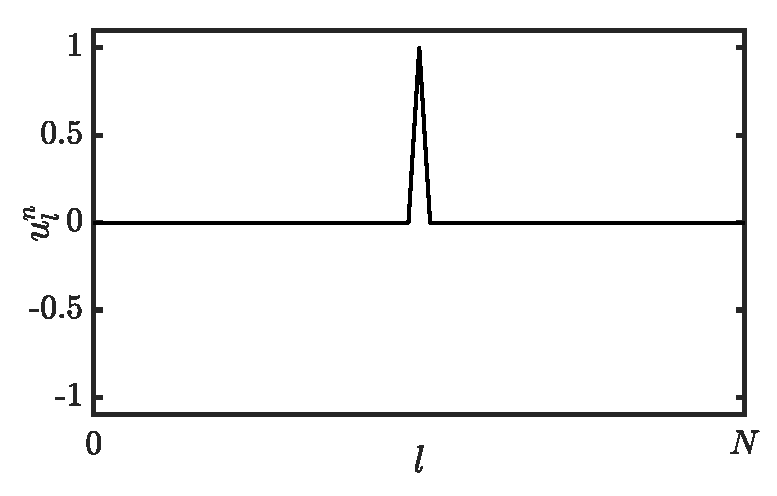
\includegraphics[width=\figWidth\textwidth]{figures/exciters/physInsp/impulse1.eps}}\hfill
    \subfloat[$n = 6$.\label{fig:impulse2}]{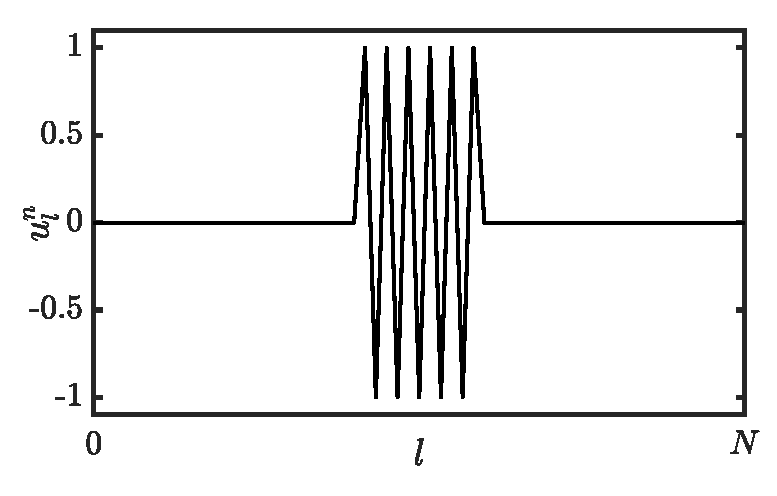
\includegraphics[width=\figWidth\textwidth]{figures/exciters/physInsp/impulse2.eps}}\hfill
    \subfloat[$n = 11$.\label{fig:impulse3}]{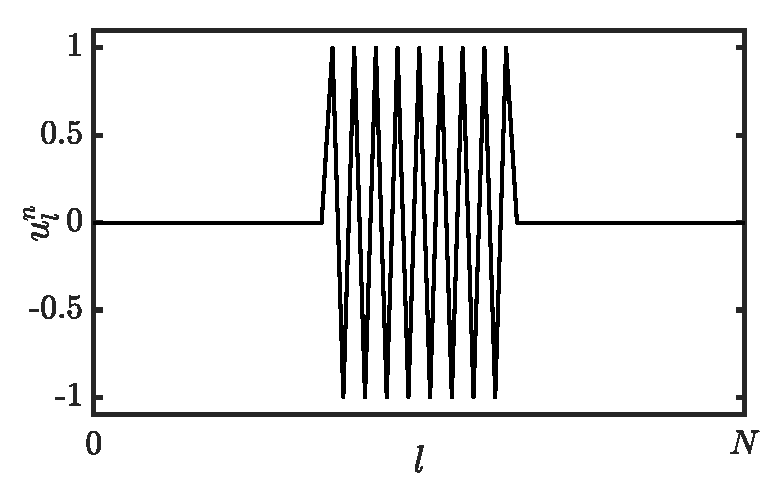
\includegraphics[width=\figWidth\textwidth]{figures/exciters/physInsp/impulse3.eps}}
    \caption{The 1D wave equation initialised with an impulse at $l=0.5N$.\label{fig:impulse}}
\end{figure}

\subsection{Raised cosine}\label{sec:raisedCosine}
The high-frequency behaviour of the impulse can be avoided by using an excitation that is spatially smooth. To achieve this, a \textit{raised cosine} is most often used due to this property and is extensively used throughout the literature \cite{theBible}. Initialising the displacement of a distributed system with a raised cosine can be interpreted as a pluck, due to the displacing and letting go. A different pluck excitation is presented in Section \ref{sec:pluck}.

A raised cosine is parametrised by its amplitude $e_\text{amp}$, its center location $x_0$ and its width $x_\text{w}$. Applied to a distributed 1D system defined over domain $x\in \D$, the (continuous-time) excitation function containing a raised cosine is defined as 
\begin{equation}\label{eq:raisedCosCont}
    e_\text{rc}(x) = 
    \begin{cases}
        \frac{e_\text{amp}}{2}\left(1 - \cos\left(\frac{2\pi (x - x_\stxt)}{x_\text{w}}\right)\right), & \text{if } x_\stxt \leq x < x_\etxt,\\
        0, & \text{otherwise},
    \end{cases}
\end{equation}
where 
\begin{equation}\label{eq:xsxe}
    x_\stxt = x_0 - 
    \frac{x_\text{w}}{2}, \qaq x_\etxt = x_0 + \frac{x_\text{w}}{2}
\end{equation}
are the start and end locations of the excitation. Furthermore, $x_\stxt, x_\etxt \in \D$ which puts a constraint on the width and location of the excitation. 

In discrete time, the center location is defined as $l_0 = \floor[x_0 / h]$, where $\floor[\cdot]$ denotes the flooring operation, $h$ is the grid spacing, and the start and end locations of the raised cosine are
\begin{equation}\label{eq:lsle}
    l_\text{s} = l_0 - \floor[w/2]\qaq l_\etxt = l_0 + \floor[w/2],
\end{equation}
and $l_\stxt, l_\etxt\in d$. Finally, $w = \floor[x_\text{w} / h]$ is the width of the excitation in grid points. A discrete raised cosine can then be created as
\begin{equation}\label{eq:raisedCosDisc}
    E_{l, \text{rc}} =
    \begin{cases}
        \frac{e_\text{amp}}{2}\left(1 - \cos\left(\frac{2\pi (l - l_\stxt)}{w-1}\right)\right), & \text{if } l_\stxt \leq l < l_\etxt,\\
        0, & \text{otherwise}.
    \end{cases}
\end{equation}
Figure \ref{fig:raisedCos} shows the 1D wave equation initialised with a raised cosine. Notice that the behaviour is much more smooth than the impulse shown in Figure \ref{fig:impulse}.

\def\figWidth{0.32}
\begin{figure}[h]
    \centering
    \subfloat[$n = 1$.\label{fig:raisedCos1}]{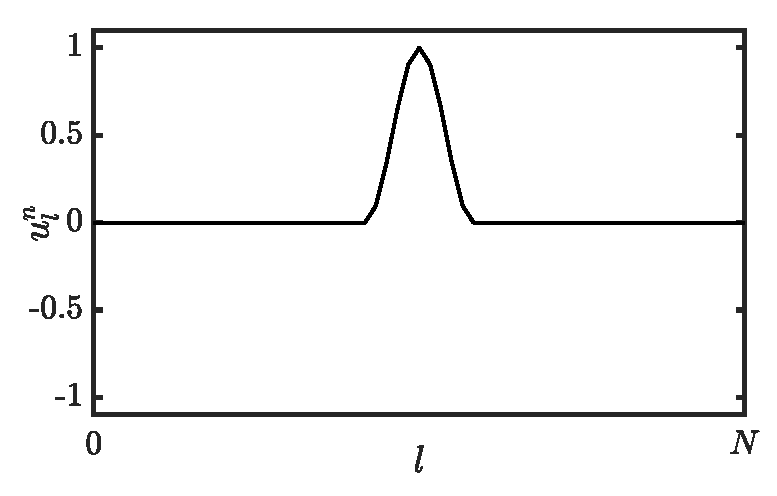
\includegraphics[width=\figWidth\textwidth]{figures/exciters/physInsp/raisedCos1.eps}}\hfill
    \subfloat[$n = 6$.\label{fig:raisedCos2}]{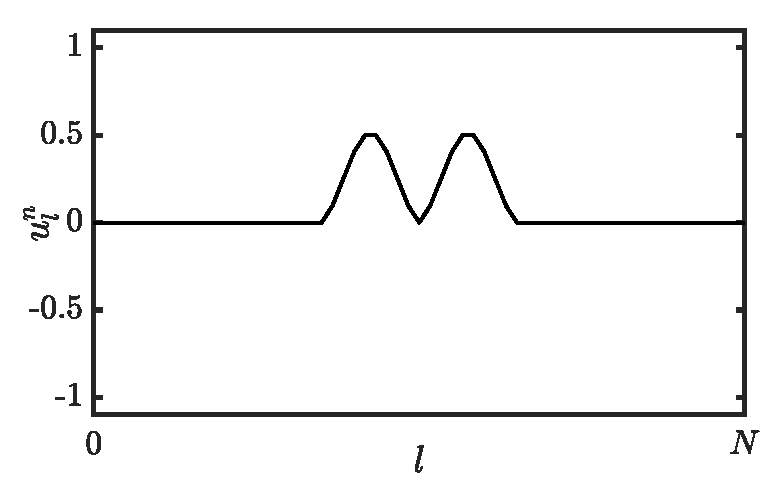
\includegraphics[width=\figWidth\textwidth]{figures/exciters/physInsp/raisedCos2.eps}}\hfill
    \subfloat[$n = 11$.\label{fig:raisedCos3}]{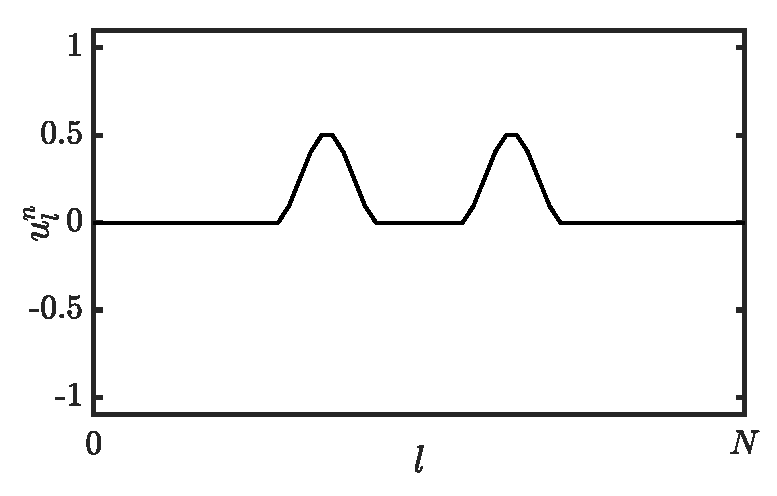
\includegraphics[width=\figWidth\textwidth]{figures/exciters/physInsp/raisedCos3.eps}}
    \caption{The 1D wave equation initialised with a raised cosine at $l_0=\floor[0.5N]$ with $e_\text{amp} = 1$.\label{fig:raisedCos}}
\end{figure}

\subsubsection{Strike}\label{sec:strike}
If one initialises the system at $n=1$ and leaves $u^0_l = 0$, one can use the raised cosine to model a strike. As can be observed from Figure \ref{fig:strike}, the amplitude of the displacement will be higher than if $u_0^n$ and $u_1^n$ were set to be the same value.\footnote{In the case of the 1D wave equation struck using a raised cosine, the maximum amplitude can be calculated to be half of the summed values of the excitation.}

\def\figWidth{0.32}
\begin{figure}[h]
    \centering
    \subfloat[$n = 1$.\label{fig:strike1}]{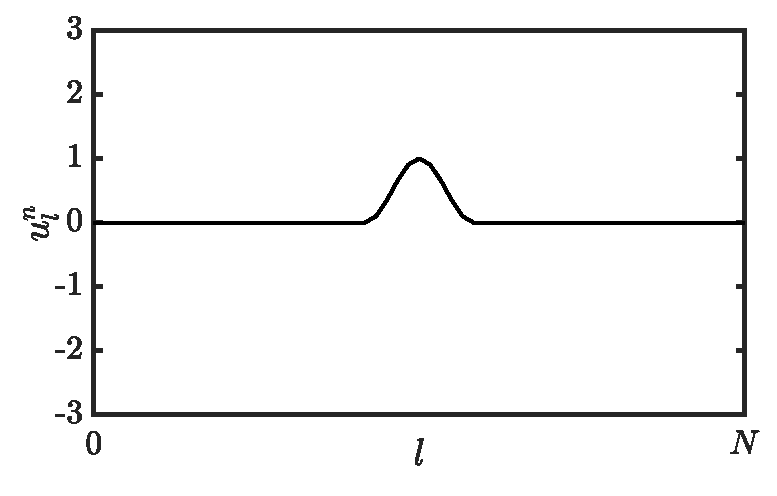
\includegraphics[width=\figWidth\textwidth]{figures/exciters/physInsp/strike1.eps}}\hfill
    \subfloat[$n = 6$.\label{fig:strike2}]{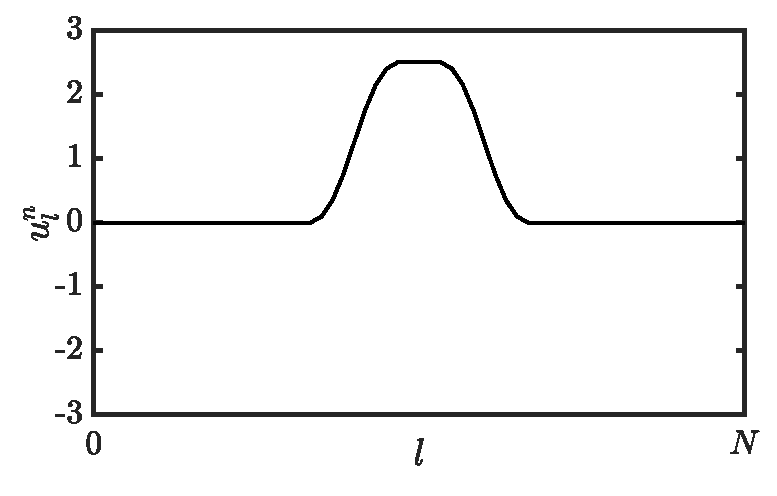
\includegraphics[width=\figWidth\textwidth]{figures/exciters/physInsp/strike2.eps}}\hfill
    \subfloat[$n = 11$.\label{fig:strike3}]{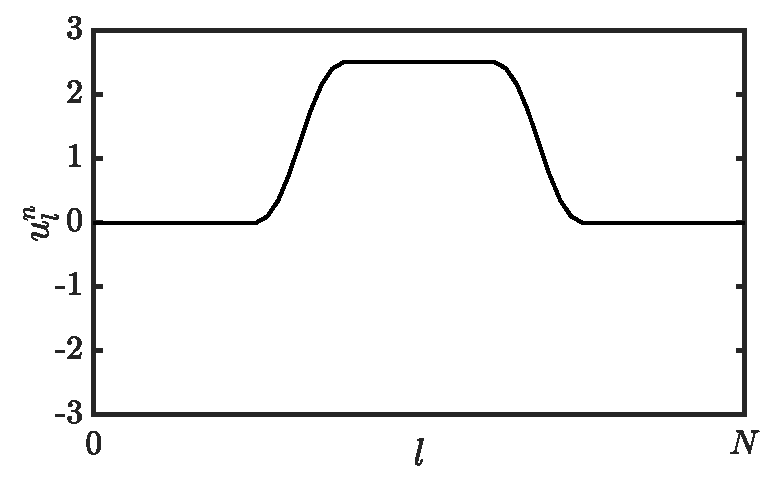
\includegraphics[width=\figWidth\textwidth]{figures/exciters/physInsp/strike3.eps}}
    \caption{The 1D wave equation initialised with a strike at $l_0=\floor[0.5N]$ with $e_\text{amp} = 1$. Notice the scaling of the y-axis compared to the other figures. \label{fig:strike}}
\end{figure}

\subsection{Triangular pluck}\label{sec:pluck}
Another initial condition for the string, which is physically more true,\todo{wording} is using a triangular shape to model a pluck. This excitation appeared in \cite{Fletcher1998}, where the authors analytically decompose the system into its modes of vibration as well as their respective amplitudes depending on the plucking position. 

Using $e_\text{amp}$ as the displacement of the corner of the triangle, and $x_0\in \D$ as the plucking position, the triangular excitation can be defined as
\begin{equation}\label{eq:triangleCont}
    e_\text{tri}(x) = \begin{cases}
        \frac{e_\text{amp}}{x_0} x, & \text{if } 0\leq x \leq x_0,\\
        \frac{e_\text{amp}}{x_0 - L} (x - L), &\text{if } x_0 < x \leq L.
    \end{cases}
\end{equation}

In discrete time, Eq. \eqref{eq:triangleCont} becomes 
\begin{equation}
    E_{l, \text{tri}} = \begin{cases}
        \frac{e_\text{amp}}{l_0} l, & \text{if } 0\leq l \leq l_0,\\
        \frac{e_\text{amp}}{l_0 - N} (l - N), &\text{if } l_0 < l \leq N.
    \end{cases}
\end{equation}
Due to the spatial discontinuity at the corner, some high-frequency oscillations (similar to the impulse) might emerge. Figure \ref{fig:pluck} shows an implementation of the 1D wave equation initialised with a triangular pluck excitation. The sample rate is 10x the usual one to prevent these high-frequency oscillations from appearing in the plot (though they still exist to some degree). 

\def\figWidth{0.32}
\begin{figure}[h]
    \centering
    \subfloat[$n = 1$.\label{fig:pluck1}]{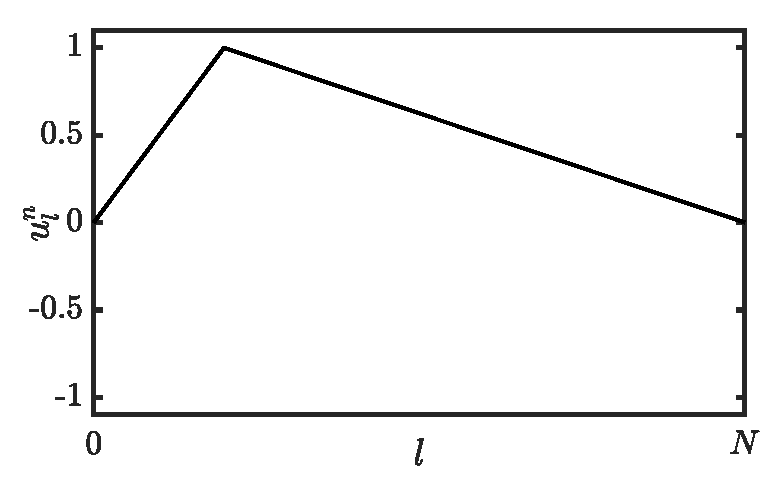
\includegraphics[width=\figWidth\textwidth]{figures/exciters/physInsp/triangle1.eps}}\hfill
    \subfloat[$n = 101$.\label{fig:pluck2}]{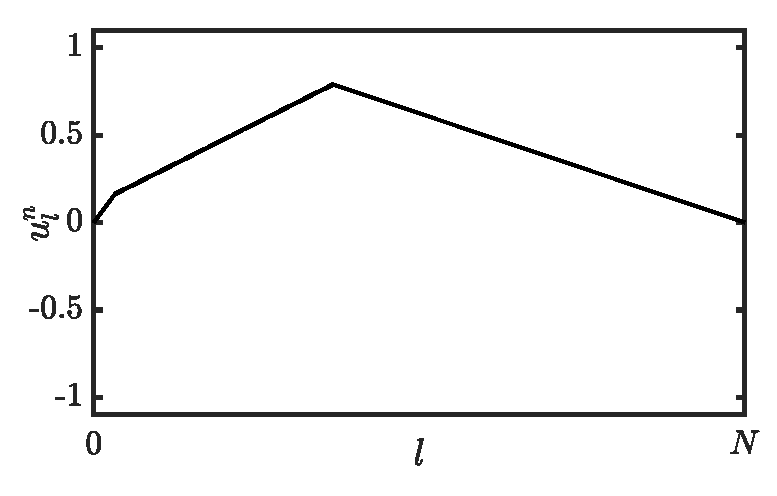
\includegraphics[width=\figWidth\textwidth]{figures/exciters/physInsp/triangle2.eps}}\hfill
    \subfloat[$n = 201$.\label{fig:pluck3}]{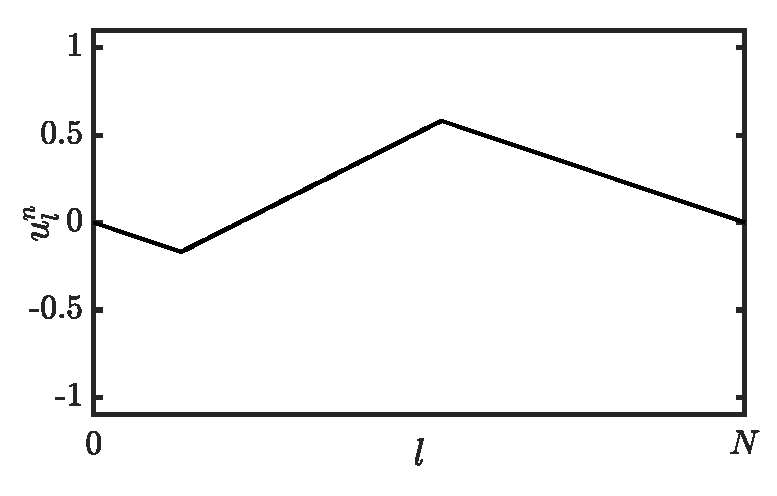
\includegraphics[width=\figWidth\textwidth]{figures/exciters/physInsp/triangle3.eps}}
    \caption{The 1D wave equation initialised with a triangular pluck with $l_0=\floor[0.2N]$. Note that sample rate has been set to $\fs = 441000$ Hz to show more ideal triangular motion. \label{fig:pluck}}
\end{figure}

\subsection{2D raised cosine}
Introducing an extra coordinate $y$, one can extend the raised cosine presented in Section \ref{sec:raisedCosine} to 2D according to 
\begin{equation}\label{eq:raisedCosCont2D}
    e_\text{rc}(x,y)\! =\! 
    \begin{cases}
        \!\frac{e_\text{amp}}{2}\left(1 - \cos\left(\frac{2\pi (x - x_\stxt)}{r_\text{w}}\right)\right)\left(1 - \cos\left(\frac{2\pi (y - y_\stxt)}{r_\text{w}}\right)\right), & 
        \!\!\!\begin{aligned}
            &\text{if } x_\stxt \leq x < x_\etxt, \\
            &\text{and } y_\stxt \leq y < y_\etxt,
        \end{aligned}\\
        \!0, &\!\! \text{otherwise},
    \end{cases}
\end{equation}
where $r_\text{w}$ is the excitation radius. Similar to Eq. \eqref{eq:xsxe}, using the center coordinate $(x_0, y_0)$, the start and end locations of the raised cosine in the $x$ and $y$ direction can be calculated as
\begin{equation*}
    x_\stxt = x_0 - 
    \frac{r_\text{w}}{2}, \quad x_\etxt = x_0 + \frac{r_\text{w}}{2}, \quad y_\stxt = y_0 - 
    \frac{r_\text{w}}{2}, \qaq y_\etxt = y_0 + \frac{r_\text{w}}{2},
\end{equation*}
where $x_\stxt, x_\etxt, y_\stxt,  y_\text{e}\in \D$ for a 2D domain $\D$.

In discrete time, Eq. \eqref{eq:raisedCosCont2D} becomes
\begin{equation}
    E_{(l,m), \text{rc}} = 
    \begin{cases}
        \!\frac{e_\text{amp}}{2}\left(1 - \cos\left(\frac{2\pi (l \!-\! l_\stxt)}{r-1}\right)\right)\!\left(1\! -\! \cos\left(\frac{2\pi (m - m_\stxt)}{r-1}\right)\right)\!, & \!\!\!\!
        \begin{aligned}
            &\text{if } l_\stxt \leq l < l_\etxt, \text{ and}\\
            & m_\stxt \leq m < m_\etxt,
        \end{aligned}\\
        \!0, &\!\!\!\! \text{otherwise},
    \end{cases}
\end{equation}
where $r = \floor[r_\text{w} / h]$ is the discrete excitation radius in grid points. Furthermore, similar to Eq. \eqref{eq:lsle},
\begin{equation}
    l_\text{s} = l_0 - \floor[r/2],\ l_\etxt = l_0 + \floor[r/2],\ m_\text{s} = m_0 - \floor[r/2], \ \text{and} \ m_\etxt = m_0 + \floor[r/2]
\end{equation}
for center coordinate $(l_0, m_0)$. 
As in the 1D case, this excitation can be used to model a simple `pluck' and strike for a 2D system. 
A simple way to implement the 2D raised cosine in \texttt{MATLAB} using the \texttt{hann} function is shown in Algorithm \ref{alg:2DraisedCos}.

\begin{lstlisting}[caption={\texttt{MATLAB} implementation of a 2D raised cosine}, label=alg:2DraisedCos]
% Assuming Dirichlet boundary conditions and having initialised the following
% - center locations for the x and y-directions: l0 and m0
% - radius of the excitation r (in grid points)

ls = l0 - floor(r/2); % start location x-direction
le = l0 + floor(r/2); % end location x-direction
ms = m0 - floor(r/2); % start location y-direction
me = m0 + floor(r/2); % end location x-direction

% Create excitation matrix
e = zeros(Ny-1, Nx-1);
e(ms:me, ls:le) = hann(rwDisc) * hann(rwDisc)';

% Applying excitation to stacked matrix form as in Section %*\refMatlab[sec:2DwaveImplementation]*)
u = reshape(e, (Nx-1) * (Ny-1), 1);
\end{lstlisting} 

\section{Time-varying excitations}
Even though the initial conditions presented in the previous section are already able to model various types of excitations, they are temporally rigid. In other words, the time of excitation is fixed to be at the start of the simulation. In order to excite the system while the simulation is running, one can create excitations that a temporal profile as well.

For the following, consider the ideal string of length $L$ (in m), its transverse displacement described by $u = u(x,t)$ (in m). The string is defined for $t\geq 0$ and $x\in\D$ with domain $\D = [0, L]$. The PDE of the ideal string with a time varying external force $f(t)$ (in N) is defined as (Eq. \eqref{eq:1DwavePDE})
\begin{equation}
    \rho A\ptt u = T \dxx u + e(x)f(t)
\end{equation}
where $e(x)$ is a spatial distribution function such as those presented in Section \ref{sec:initConditionsPhysInsp}.

\subsection{Raised cosine}
To yield a smooth excitation over time, one can, similar to the spatially distributed raised cosine in Eq. \ref{sec:raisedCosine}, define a temporally distributed raised cosine. Using the time of excitation $t_0\geq 0$ and excitation duration $t_\text{d}>0$ (both in s) the temporal raised cosine can be used as a force function, as
\begin{equation}\label{eq:raisedCosTemp}
    f(t) = 
    \begin{cases}
        \frac{f_\text{amp}}{2} \left(1 - \cos\left(\frac{q\pi (t - t_0)}{t_\text{d}}\right)\right), & t_\stxt \leq t < t_0 + t_\text{d}\\
        0, &\text{otherwise}.
    \end{cases}
\end{equation} 
As done in \cite{Webb2015}, $q$ that alters the excitation to be a pluck when $q=1$ and a strike when $q=2$. Finally, $f_\text{amp}$ is the maximum force (in N). 

As done in papers \citeP[A] and \citeP[B], the force function can be used in conjunction with the distribution functions shown in Section \ref{sec:initConditionsPhysInsp}. When used to scale a spatially distributed raised cosine in Eq. \eqref{eq:raisedCosCont}, one can model a pluck ($q=1$) and a strike ($q=2$). These alternatives are visualised in Figure \ref{fig:timeVaryingRaisedCos}. Note that one would like $f_\text{amp}$ to be the maximum force, one must set $e_\text{amp} = 1$ in Eq. \eqref{eq:raisedCosCont} such that the maximum force can be controlled using $f_\text{amp}$. 

In discrete time, the force function in Eq. \eqref{eq:raisedCosTemp} becomes
\begin{equation}\label{eq:discExcitation}
    f^n = 
    \begin{cases}
        \frac{f_\text{amp}}{2}\left(1-\cos\left(\frac{q\pi (n - n_0)}{n_\text{d}}\right)\right), & n_0 \leq n < n_0+n_\text{d},\\
        0, &\text{otherwise}.
    \end{cases}
\end{equation}



\def\figWidth{0.8}
\begin{figure}[h]
    \centering
    \subfloat[Pluck ($q=1$).\label{fig:timeVaryingRaisedCosPluck}]{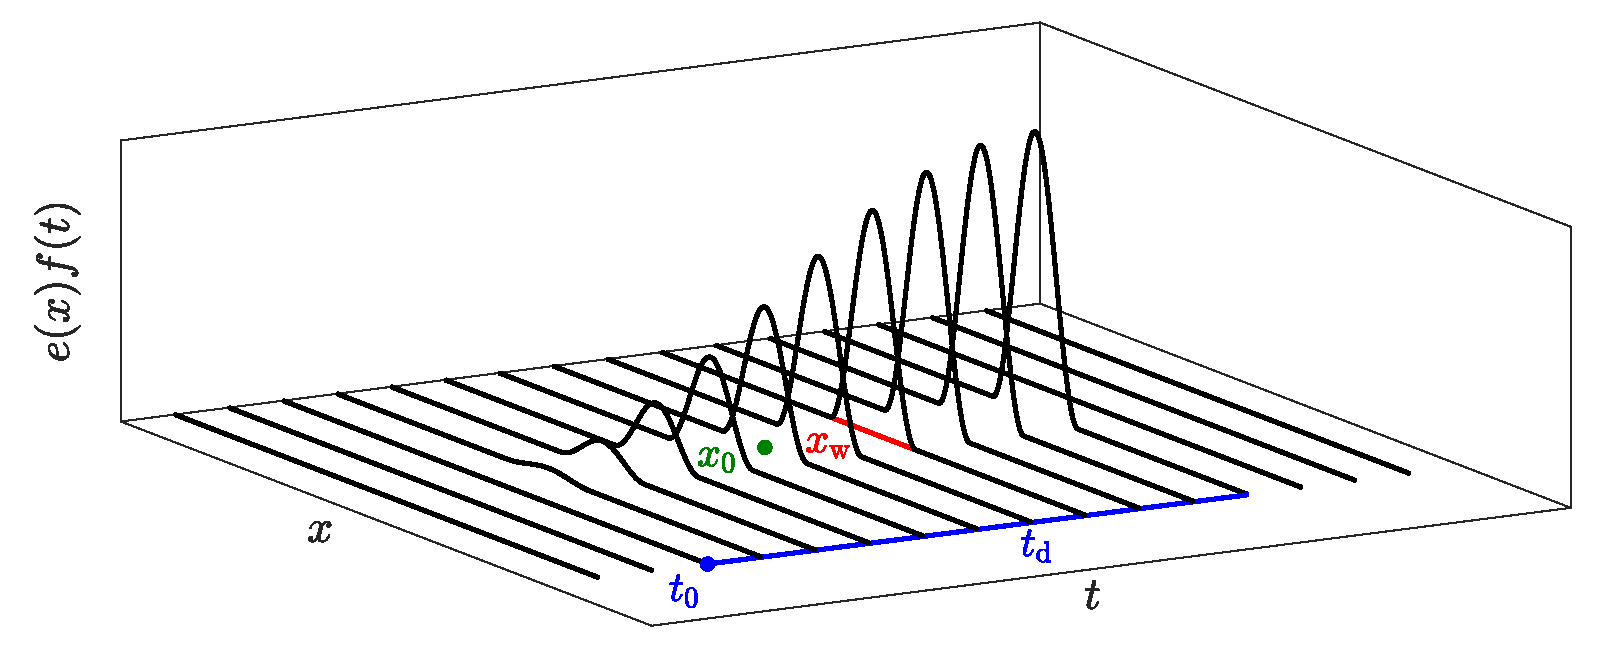
\includegraphics[width=\figWidth\textwidth]{figures/exciters/physInsp/timeVaryingRaisedCos.eps}}\\
    \subfloat[Strike ($q=2$).\label{fig:timeVaryingRaisedCosStrike}]{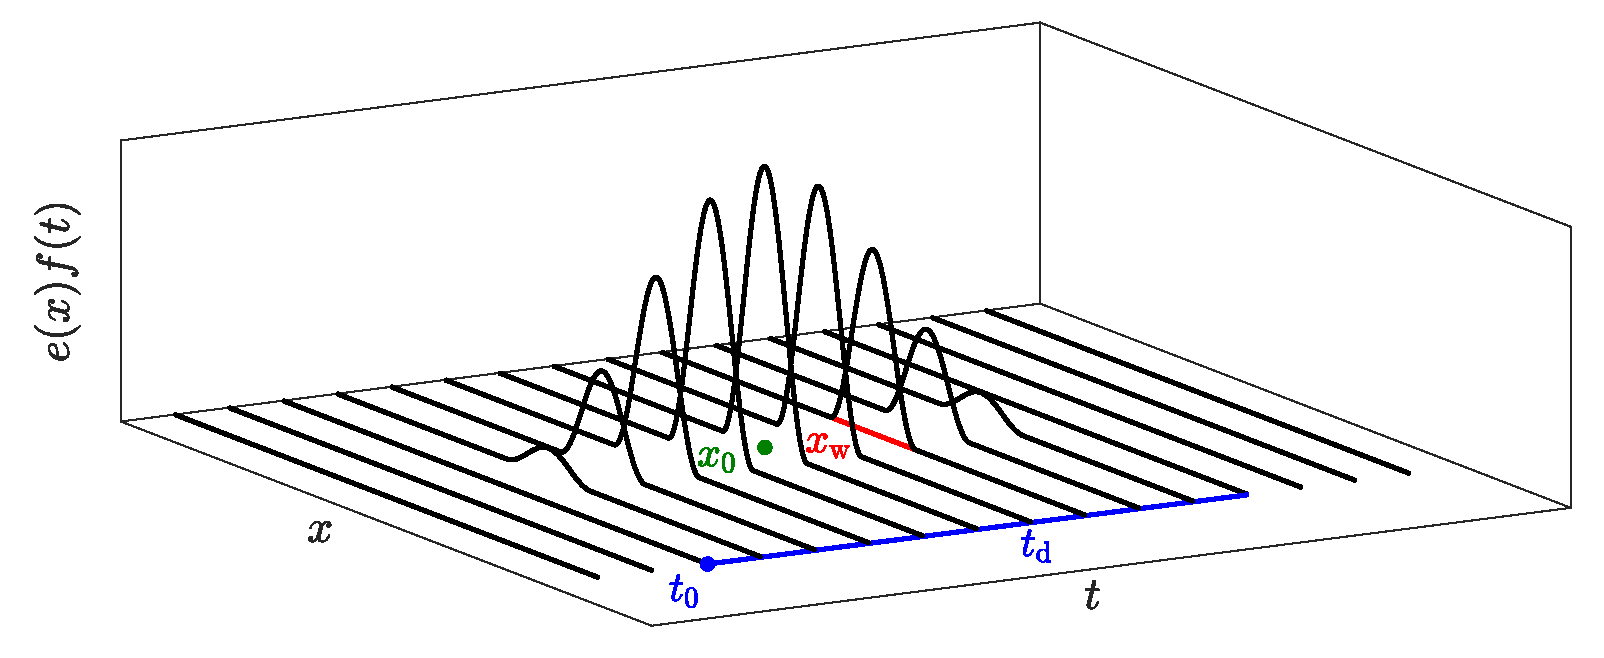
\includegraphics[width=\figWidth\textwidth]{figures/exciters/physInsp/timeVaryingRaisedCosHammer.eps}}\hfill
    \caption{The time-varying raised cosine showing a (a) pluck and a (b) strike. The location of excitation $x_0$ is shown in green, the width $x_\text{w}$ in red and the excitation start $t_0$ and duration $t_\text{d}$ in blue.\label{fig:timeVaryingRaisedCos}}
\end{figure}

\subsection{Pulse train}\label{sec:pulseTrain}
As already briefly introduced in Section \ref{sec:webstersExcitation}, one can create a pulse train to excite an acoustic tube. This is inspired by \cite{theBible} where the signal represents the opening and closing of the glottis. As the characteristics of the lip reed are similar to the vocal folds \cite{Richards2003}, the pulse train has been used as a test signal here. A more complete model of the lip reed can be found in Chapter \ref{ch:lipreed}.

The pulse train can be created using a clipped sinusoid which can be used as the input velocity to an acoustic tube. For a pulse train with a maximum amplitude of 1 and a frequency $f$ (in Hz), the following is proposed
\def\depth{c_\text{d}}
\begin{equation}\label{eq:pulseTrain}
    v_\text{in} = \left[\frac{\sin(2\pi f t) - (1-2\depth)}{2\depth}\right]_+,
\end{equation}
where $0< \depth \leq 0.5$ is the clipping depth, and determines the duty cycle, i.e. the distance between the pulses. Finally, the $[\cdot]_+$ operator specifies `the positive part of' and is used for clipping (see Chapter \ref{ch:collisions}). See Figure \ref{fig:pulseTrain} for an example. 

\begin{figure}[h]
    \centering
    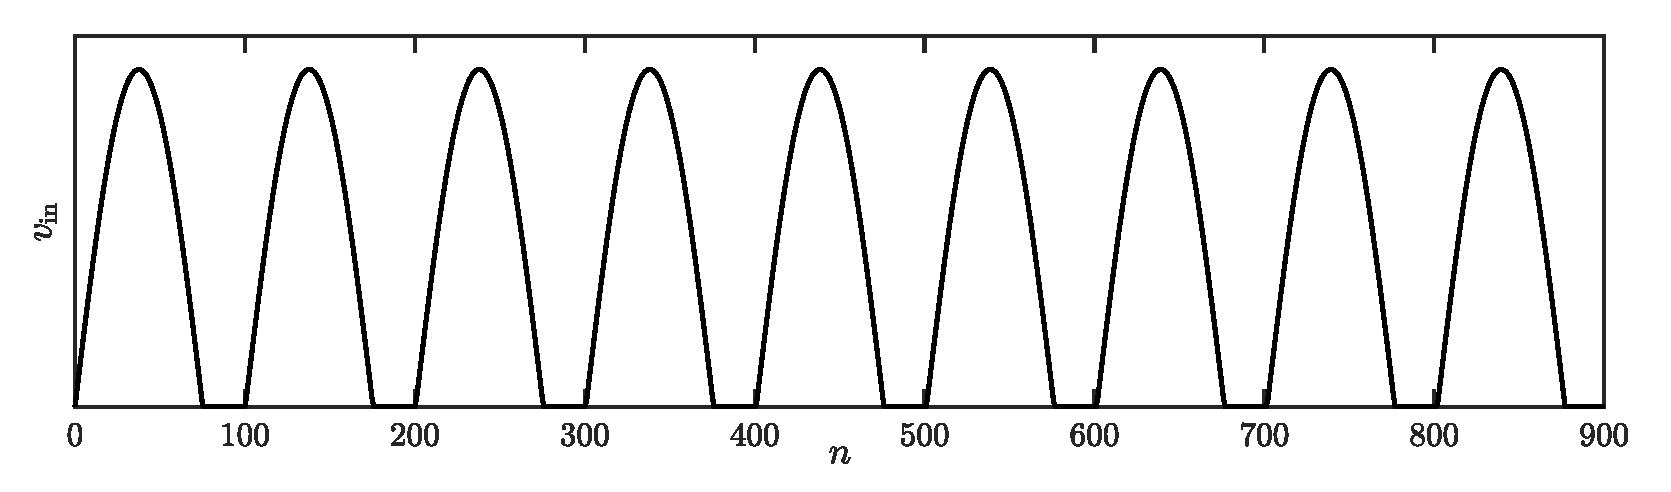
\includegraphics[width=\textwidth]{figures/exciters/physInsp/pulseTrain.eps}
    \caption{Example of a pulse train using Eq. \eqref{eq:pulseTrain} with $f=100$ Hz and $\depth = 0.25$.
    \label{fig:pulseTrain}}
\end{figure}